\documentclass{article}
%\documentclass[journal]{IEEEtran}
%\documentclass{report}
%\documentclass{ActaOulu}

\usepackage{graphicx}
\usepackage{listings}
\usepackage{amsmath}

\begin{document}

\title{Report of Project 4}
\author{Wei Jiang}

\maketitle

\begin{abstract}
The Project 4 of PHY607 has only 1 exercises.
The goal of this project is to solve a one dimensional simple harmonic potential.
\end{abstract}


%\chapter{First Chapter}

\section{Introduction}

This exercise asks us to solve schrodinger equation for one dimensional simple harmonic potential. We set k, m, $\hbar$ equal one. The method we use is Numerov algorithm to solve this differential equation, and compare with analytical solutions.


\section{Conclusion}
\subsection{Strategy and code}
In this exercise, the equation we need to solve is 
\begin{equation}
\left( -\frac{\hbar}{2 m}\frac{d^2}{dx^2} + \frac{1}{2} k x^2 \right)\psi = E\psi
\end{equation}
If we set the parameters $m$, $\hbar$, $k$ equal one, the equation becomes
\begin{equation}\label{scheq}
\frac{d^2\psi}{dx^2} + \left( E - V \right)\psi = 0.
\end{equation}
For a general differential equation, the form of equation is 
\begin{equation}
\frac{d^2}{dx^2} y(x) =f (x, y(x)).
\end{equation}
Then according to the hangout in class, the solution for $y_n(x)$ is
\begin{equation}
\left(1+\frac{h^2}{12}f_{n+1}\right)y_{n+1} = \left(2 - \frac{5h^2}{12}f_n \right)y_n - \left(1 + \frac{h^2}{12}f_{n-1}\right)y_{n-1}.
\end{equation}
So the eigenstate of Eq.\ref{scheq} is
\begin{equation}\label{recur}
\left(1 - \frac{h^2}{12}f_{i+1}\right)\psi_{i+1} = \left(2 + \frac{5}{6} h^2 f_i \right)\psi_i - \left(1 - \frac{h^2}{12}f_{i-1}\right)\psi_{i-1}.
\end{equation}
Because the hangout ask use even and odd function to solve the equation, they have different boundary condition,
We define even and odd function as:
\begin{equation}
\psi(0) = 1, \psi(h) = 1 + \frac{h^2}{2}f(0) + \frac{h^4}{24}(f''(0) + f^2(0)) ; even solutions
\end{equation}
\begin{equation}
\psi(0) = 0, \psi(h) = h + \frac{h^3}{6}f(0) ;  odd solutions
\end{equation}

Then we can repeat Eq.\ref{recur} to get more data, the code is shown below
\begin{lstlisting}
#include <stdio.h>
#include <gsl/gsl_math.h>
#include <time.h>
#include <gsl/gsl_matrix.h>
#include <gsl/gsl_rng.h>
#include <gsl/gsl_permutation.h>
#include <gsl/gsl_linalg.h>

/* Dimension of Matrix and Vectors */

int main(void)
{
    
    /*int i, j;*/
    const gsl_rng_type * T;
    gsl_rng * r;
    
    gsl_rng_env_setup();
    T = gsl_rng_default;
    r = gsl_rng_alloc (T);
    int s;
    double det;
 
    double n = 500.0;
    
    FILE *fp;
    fp = fopen( "output.txt", "w" );
    for (int i = 0; i < 4; i ++) {
        clock_t start, finish;
        double  duration;
        /* duration of program */
        start = clock();
        
        gsl_matrix *m = gsl_matrix_alloc(n, n);
        
        for (int inter = 0; inter < n; inter++) {
            for (int inter2 = 0; inter2 < n; inter2++) {
                double u = gsl_rng_uniform (r);
                gsl_matrix_set(m, inter, inter2, u);
            }
        }
        
        gsl_permutation*p = gsl_permutation_calloc(n);
        gsl_linalg_LU_decomp (m, p, &s);
        det = gsl_linalg_LU_det(m, s);
        finish = clock();
        duration = (double)(finish - start) / CLOCKS_PER_SEC;
        printf( "%e %f seconds\n",log(n), log(duration) );
        fprintf(fp, "%e %e\n",log(n), log(duration));
        n = n + 500;
        gsl_permutation_free(p);
        gsl_matrix_free (m);
    }
    fclose( fp );
    gsl_rng_free (r);
    return 0;
}
\end{lstlisting} 

\subsection{Test for result}
To test if our numerical solution is correct, we need to compare with analytic solution. we plot ground state and first exited state in Fig.\ref{ground} and Fig.\ref{exited}. They are same curve, although they have different scalings.
\begin{figure}
    \centering
    \includegraphics[width=2.3in]{ground_num.eps}
    \includegraphics[width=2.3in]{ground_asol.eps}
    \caption{Ground state of harmonic oscillator. Left: numerical solution; Right:  analytic solution}
    \label{ground}
\end{figure}
\begin{figure}
    \centering
    \includegraphics[width=2.3in]{1st_num.eps}
    \includegraphics[width=2.3in]{1st_asol.eps}
    \caption{Exited state of harmonic oscillator. Left: numerical solution; Right:  analytic solution}
    \label{exited}
\end{figure}

\subsection{Change parameter}
If we change our parameter, $h=0.05$, $x = 5$, set $E = 0.95$, $E = 1.0$ and $E = 1.05$, and plot them in Fig.\ref{echange}. We find that the curve sensitive to energy, energy change a little bit, but eigenstate change a lot.
\begin{figure}
    \centering
    \includegraphics[width=1.5in]{e0.eps}
    \includegraphics[width=1.5in]{ground_num.eps}
    \includegraphics[width=1.5in]{e1.eps}
    \caption{Ground state of harmonic oscillator. Left: E = 0.95; Center: E = 1; Right:  E = 1.05}
    \label{echange}
\end{figure}

I guess the reason comes from Eq.\ref{scheq}, the coefficient of $\psi_{i+1}$ is depends on E and x. If E change or x increase the curve can change strikingly. So we increase x to a large number, we find that eigenfunction is very different from analytic solution and plot them in Fig.\ref{xlarge}.
\begin{figure}
    \centering
    \includegraphics[width=2.3in]{largex.eps}
    \includegraphics[width=2.3in]{ground_num.eps}
    \caption{Ground state of harmonic oscillator. Left: up band of x is 5; Right:  up band of x is 6.5. Left graph diverse at large x, but Right graph goes to zero, which is correct for ground state}
    \label{xlarge}
\end{figure}

\subsection{Solutions of E = 3, 5 and 7}
Finally, we plot the solution of E = 3, 5 and 7. We know that the eigenstate of E = 3, 5, 7 should be odd function, even function and odd function. The graph is shown in Fig.\ref{eigens}, it is self consist with our exception.

\begin{figure}
    \centering
    \includegraphics[width=1.5in]{n=1.eps}
    \includegraphics[width=1.5in]{n=2.eps}
    \includegraphics[width=1.5in]{n=3.eps}
    \caption{Eigenstate of E = 3, 5, 7}
    \label{eigens}
\end{figure}


\end{document}
